\pagestyle{empty}
\chapter*{ПРИЛОЖЕНИЯ}
\addcontentsline{toc}{chapter}{ПРИЛОЖЕНИЯ}

\begin{flushright}
\phantomsection
\appendix{ПРИЛОЖЕНИЕ} \textlabel{app:masks}{А}
\addcontentsline{toc}{section}{ПРИЛОЖЕНИЕ А}
\end{flushright}
\begin{center}
Статья о капитализме
\end{center}
Capitalism is an economic system based on the private ownership of the means of production and their operation for profit. Characteristics central to capitalism include private property, capital accumulation, wage labor, voluntary exchange, a price system and competitive markets. In a capitalist market economy, decision-making and investments are determined by every owner of wealth, property or production ability in financial and capital markets whereas prices and the distribution of goods and services are mainly determined by competition in goods and services markets.

Economists, political economists, sociologists and historians have adopted different perspectives in their analyses of capitalism and have recognized various forms of it in practice. These include laissez-faire or free-market capitalism, welfare capitalism and state capitalism. Different forms of capitalism feature varying degrees of free markets, public ownership, obstacles to free competition and state-sanctioned social policies. The degree of competition in markets, the role of intervention and regulation, and the scope of state ownership vary across different models of capitalism. The extent to which different markets are free as well as the rules defining private property are matters of politics and policy. Most existing capitalist economies are mixed economies which combine elements of free markets with state intervention and in some cases economic planning.

Market economies have existed under many forms of government and in many different times, places and cultures. Modern capitalist societies—marked by a universalization of money-based social relations, a consistently large and system-wide class of workers who must work for wages, and a capitalist class which owns the means of production—developed in Western Europe in a process that led to the Industrial Revolution. Capitalist systems with varying degrees of direct government intervention have since become dominant in the Western world and continue to spread. Over time, capitalist countries have experienced consistent economic growth and an increase in the standard of living.

Critics of capitalism argue that it establishes power in the hands of a minority capitalist class that exists through the exploitation of the majority working class and their labor; it prioritizes profit over social good, natural resources and the environment; and it is an engine of inequality, corruption and economic instabilities. Supporters argue that it provides better products and innovation through competition, disperses wealth to all productive people, promotes pluralism and decentralization of power, creates strong economic growth and yields productivity and prosperity that greatly benefit society.


\thispagestyle{empty}
\newpage

\begin{flushright}
\phantomsection
\appendix{ПРИЛОЖЕНИЕ} \textlabel{app:harry}{Б}
\end{flushright}
\begin{center}
Часть первой главы книги Гарри Поттер
\end{center}

The Dursleys are a well-to-do, status-conscious family living in Surrey, England. Eager to keep up proper appearances, they are embarrassed by Mrs. Dursley’s eccentric sister, Mrs. Potter, whom for years Mrs. Dursley has pretended not to know. On his way to work one ordinary morning, Mr. Dursley notices a cat reading a map. He is unsettled, but tells himself that he has only imagined it. Then, as Mr. Dursley is waiting in traffic, he notices people dressed in brightly colored cloaks. Walking past a bakery later that day, he overhears people talking in an excited manner about his sister-in-law’s family, the Potters, and the Potters’ one-year-old son, Harry. Disturbed but still not sure anything is wrong, Mr. Dursley decides not to say anything to his wife. On the way home, he bumps into a strangely dressed man who gleefully exclaims that someone named “You-Know-Who” has finally gone and that even a “Muggle” like Mr. Dursley should rejoice. Meanwhile, the news is full of unusual reports of shooting stars and owls flying during the day.

That night, as the Dursleys are falling asleep, Albus Dumbledore, a wizard and the head of the Hogwarts wizardry academy, appears on their street. He shuts off all the streetlights and approaches a cat that is soon revealed to be a woman named Professor McGonagall (who also teaches at Hogwarts) in disguise. They discuss the disappearance of You-Know-Who, otherwise known as Voldemort. Dumbledore tells McGonagall that Voldemort killed the Potter parents the previous night and tried to kill their son, Harry, as well, but was unable to. Dumbledore adds that Voldemort’s power apparently began to wane after his failed attempt to kill Harry and that he retreated. Dumbledore adds that the baby Harry can be left on the Dursleys’ doorstep. McGonagall protests that Harry cannot be brought up by the Dursleys. But Dumbledore insists that there is no one else to take care of the child. He says that when Harry is old enough, he will be told of his fate. A giant named Hagrid, who is carrying a bundle of blankets with the baby Harry inside, then falls out of the sky on a motorcycle. Dumbledore takes Harry and places him on the Dursley’s doorstep with an explanatory letter he has written to the Dursleys, and the three part ways.

\newpage

\begin{flushright}
\phantomsection
\appendix{ПРИЛОЖЕНИЕ} \textlabel{app:main}{В}
\addcontentsline{toc}{section}{ПРИЛОЖЕНИЕ В}
\end{flushright}
\begin{center}
Графический интерфейс главной страницы модуля mVis
\end{center}
\begin{figure}[H]
\centering
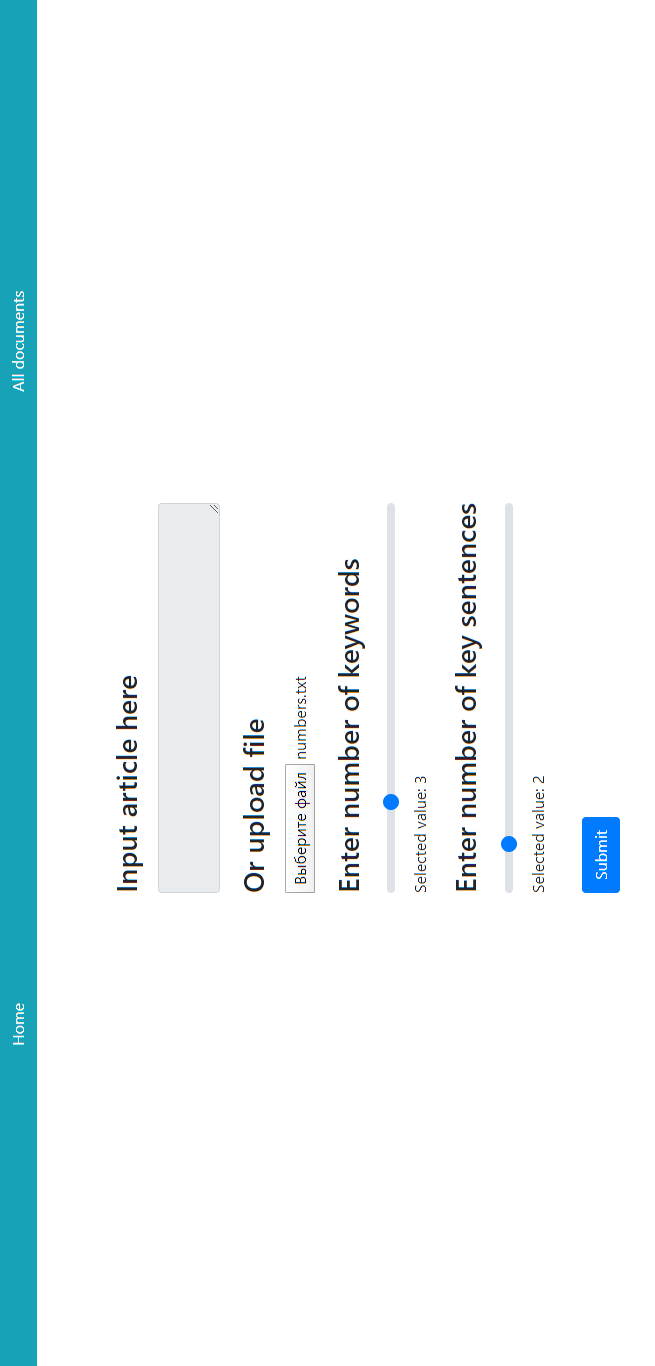
\includegraphics[height=0.8\textheight]{mainpage.png}
\end{figure}

\newpage

\begin{flushright}
\phantomsection
\appendix{ПРИЛОЖЕНИЕ} \textlabel{app:all}{Г}
\addcontentsline{toc}{section}{ПРИЛОЖЕНИЕ Г}
\end{flushright}
\begin{center}
Графический интерфейс страницы для отображения всех документов модуля mVis
\end{center}
\begin{figure}[H]
\centering
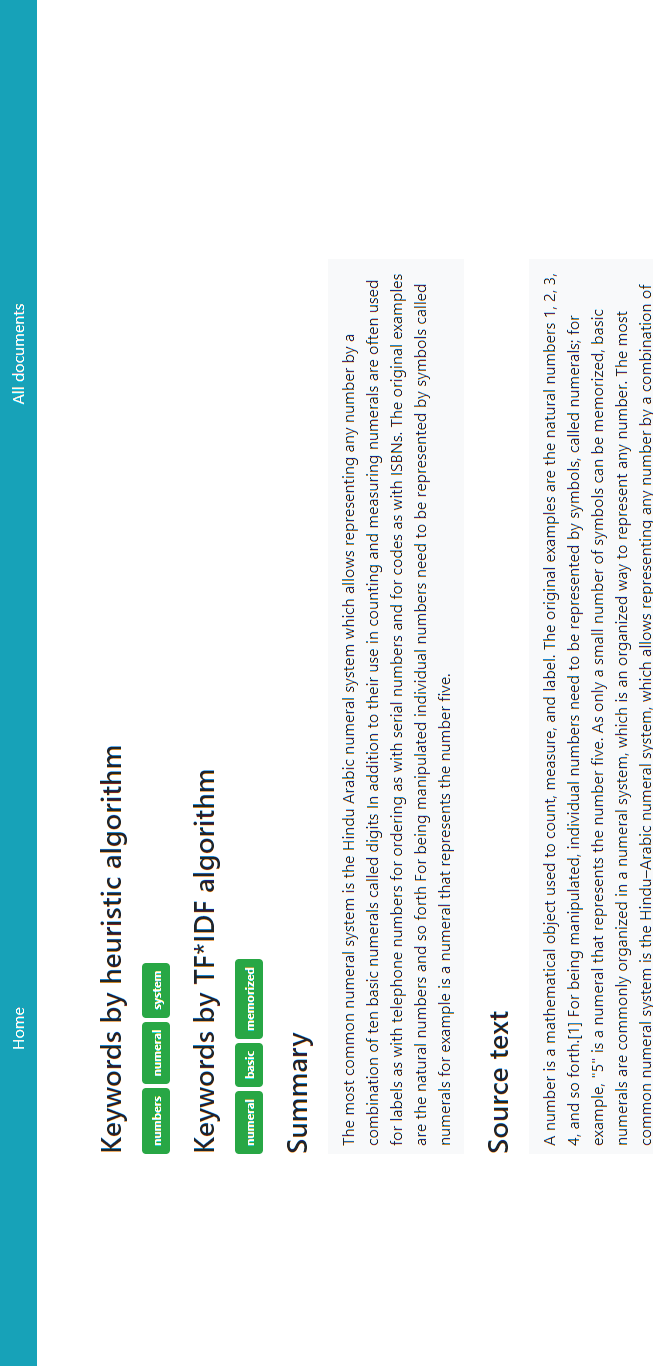
\includegraphics[height=0.85\textheight]{alldocs.png}
\end{figure}

\newpage
